% Standalone file to compile the normalize single edge TikZ figure
\documentclass[tikz,border=2mm]{standalone}
\usepackage{tikz}
\usetikzlibrary{arrows.meta,decorations.pathmorphing}
\begin{document}
% Figure content (same as fig_normalize_single_edge.tex)
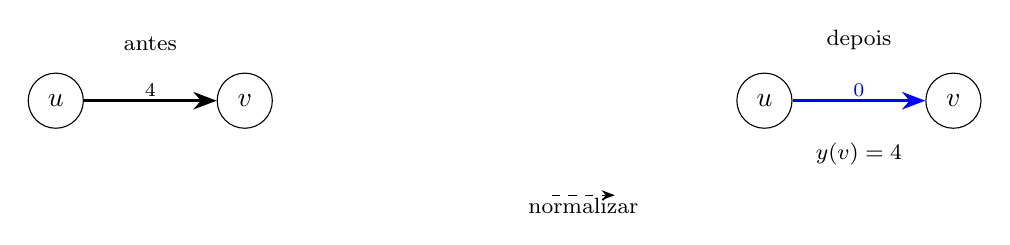
\begin{tikzpicture}[>=Stealth, node distance=2.0cm, every node/.style={inner sep=1pt}]
	% Left: original
	\begin{scope}[xshift=-4.5cm]
		\node[circle,draw,minimum size=7mm] (u) at (0,0) {$u$};
		\node[circle,draw,minimum size=7mm] (v) at (2.4,0) {$v$};
		\draw[->, very thick] (u) -- node[midway, above] {\scriptsize 4} (v);
		\node[anchor=south] at (1.2,0.6) {\footnotesize antes};
	\end{scope}

	% Right: normalized
	\begin{scope}[xshift=4.5cm]
		\node[circle,draw,minimum size=7mm] (u2) at (0,0) {$u$};
		\node[circle,draw,minimum size=7mm] (v2) at (2.4,0) {$v$};
		\draw[->, very thick, blue] (u2) -- node[midway, above, text=blue] {\scriptsize 0} (v2);
		\node[anchor=south] at (1.2,0.6) {\footnotesize depois};
		% label showing y(v)=4
		\node[anchor=north] at (1.2,-0.5) {\footnotesize $y(v)=4$};
	\end{scope}

	% Optional small explanatory arrow between pictures
	\draw[->, dashed] (1.8, -1.2) -- (2.6, -1.2) node[midway, below] {\footnotesize normalizar};
\end{tikzpicture}
\end{document}
